% !TeX document-id = {0be8c18c-9430-4e9a-bdd9-12beadebfebc}
% !TeX TXS-program:bibliography = txs:///biber
\documentclass[11pt]{beamer}

\usepackage[brazilian]{babel}

\uselanguage{portuguese}
\languagepath{portuguese}
\deftranslation[to=portuguese]{Theorem}{Teorema}
\deftranslation[to=portuguese]{theorem}{teorema}
\deftranslation[to=portuguese]{Example}{Exemplo}
\deftranslation[to=portuguese]{example}{exemplo}
\deftranslation[to=portuguese]{Lemma}{Lema}
\deftranslation[to=portuguese]{lemma}{Lema}
\deftranslation[to=portuguese]{Corollary}{Corolário}
\deftranslation[to=portuguese]{corollary}{corolário}
%\deftranslation[to=portuguese]{and}{e}
\newtheorem{proposition}{Proposição}
\newtheorem{assumption}{Hipótese}

\usepackage[utf8]{inputenc}
\usepackage[T1]{fontenc}
\usepackage{lmodern}
\usepackage{amsmath}
\usepackage{amssymb}
\usepackage{mathtools}
\usepackage{color}
\usepackage{pgfplots}
\usepackage{tikz}
\usepackage{subcaption}
%\usepackage{appendixnumberbeamer}

\newenvironment{transitionframe}{
	\setbeamercolor{background canvas}{bg=yellow}
	\begin{frame}}{
	\end{frame}
}
\usetheme{default}
\usefonttheme{structuresmallcapsserif}

%% I use a beige off white for my background
\definecolor{MyBackground}{RGB}{255,253,218}
\useinnertheme[shadow]{rounded}
\setbeamercolor{block title}{bg=MyBackground}
\setbeamercolor{block body}{bg=MyBackground}
\setbeamercolor{example title}{bg=MyBackground}
\setbeamercolor{example body}{bg=MyBackground}


\newcommand{\blue}[1]{\textcolor{blue}{#1}}
\newcommand{\red}[1]{\textcolor{red}{#1}}
\newcommand{\purple}[1]{\textcolor{purple}{#1}}
\newcommand{\gray}[1]{\textcolor{gray}{#1}}
\setbeamertemplate{navigation symbols}{}
%\setbeamertemplate{page number in head/foot}[appendixframenumber]

%\usepackage{graphics}
\usepackage{graphicx}

\definecolor{blue_emph}{RGB}{0,114,178}
\definecolor{red}{RGB}{213,94,0}
\definecolor{yellow}{RGB}{240,228,66}
\definecolor{green}{RGB}{0,158,115}
\definecolor{purple}{RGB}{204,121,167}
\definecolor{orange}{RGB}{230,159,0}
\definecolor{lightblue}{RGB}{86,180,233}

%\setbeamercolor{frametitle}{fg=blue}
%\setbeamercolor{title}{fg=blue}
\setbeamertemplate{footline}[frame number]
\setbeamertemplate{navigation symbols}{} 
\setbeamertemplate{itemize items}{-}
%\setbeamercolor{itemize item}{fg=blue}
%\setbeamercolor{itemize subitem}{fg=blue}
\setbeamertemplate{enumerate items}[default]
%\setbeamercolor{enumerate subitem}{fg=blue}
\setbeamercolor{button}{bg=MyBackground,fg=blue}
\usefonttheme{structuresmallcapsserif}

%\setbeamercolor{section in toc}{fg=blue}
%\setbeamercolor{subsection in toc}{fg=red}
\setbeamersize{text margin left=1em,text margin right=1em} 


\usepackage{appendixnumberbeamer}
\usepackage{pdfpages}
\usepackage[
backend=biber,
uniquename=false,
uniquelist=false,
style=authoryear,
natbib=true
]{biblatex}
\addbibresource{../bibliography.bib}

\newenvironment{wideitemize}{\itemize\addtolength{\itemsep}{10pt}}{\enditemize}
\newenvironment{wideenumerate}{\enumerate\addtolength{\itemsep}{10pt}}{\endenumerate}
\newenvironment{halfwideitemize}{\itemize\addtolength{\itemsep}{0.5em}}{\enditemize}
\newenvironment{halfwideenumerate}{\enumerate\addtolength{\itemsep}{0.5em}}{\endenumerate}


\author{Luis A. F. Alvarez}
\title{Econometria I}
\subtitle{O estimador de Mínimos Quadrados Ordinários}
%\logo{}
%\institute{}
\date{\today}
%\subject{}
%\setbeamercovered{transparent}

\def\signed #1{{\leavevmode\unskip\nobreak\hfil\penalty50\hskip2em
		\hbox{}\nobreak\hfil(#1)%
		\parfillskip=0pt \finalhyphendemerits=0 \endgraf}}

\newsavebox\mybox
\newenvironment{aquote}[1]
{\savebox\mybox{#1}\begin{quote}}
	{\signed{\usebox\mybox}\end{quote}}

\begin{document}

\begin{frame}[plain]
	\maketitle
\end{frame}
\begin{frame}{Ambiente}
	\begin{itemize}
		\item Pesquisador observa $n$ pares $(Y_i,X_i)$, $i=1\ldots, n$, para os quais supõe um modelo linear da forma:
		\begin{equation}
			\label{eq_line}
			Y_i = X_i'\beta + \epsilon_i\, \ldots  i=1,\ldots n\, ,
		\end{equation}
		onde $\beta\in \mathbb{R}^k$ é um parâmetro desconhecido, e $\epsilon_i$, $i=1,\ldots, n$ são variáveis aleatórias não observadas.
		\begin{itemize}
			\item Recorde-se, da última aula, que cabe ao pesquisador postular o modelo e a interpretação dos coeficientes.
			\item No caso mais comum, $(Y_i,X_i) \overset{d}{=} (Y,X)$ para $i=1,\ldots, n$, onde a distribuição de $(Y,X)$ representa a distribuição das variáveis numa população de interesse.
			\begin{itemize}
				\item Por exemplo, podemos ter que $\{(Y_i, X_i)\}_{i=1}^n$ é uma amostra aleatória de uma população com distribuição $\mathbb{P}_{Y,X}$, para a qual postulamos um modelo linear.
				\item Mas também podemos ter que as observações entre pares apresentem dependência entre si, embora com leis $\mathbb{P}_{(Y_i, X_i)}$ comuns a todo $i$.
			\end{itemize} 
			\item De modo mais geral, no entanto, pode ser que os $(Y_i,X_i)$ não possuam a mesma distribuição conjunta, mas haja uma relação comum e estável ao longo de $i$.
		\end{itemize}
	\end{itemize}
\end{frame}
\begin{frame}{Notação matricial}
	\begin{itemize}

	\item No que segue, definimos as seguintes matrizes aleatórias:
	
	$$\boldsymbol{y} = \begin{bmatrix}
		Y_1 \\
		Y_2 \\
		\vdots \\
		Y_n
	\end{bmatrix}\, , \quad \boldsymbol{X} = \begin{bmatrix}
	X_1' \\
	X_2' \\
	\vdots \\
	X_n'
	\end{bmatrix}\,, \quad \boldsymbol{\epsilon} = \begin{bmatrix}
	\epsilon_1 \\
	\epsilon_2 \\
	\vdots \\
	\epsilon_n
	\end{bmatrix}$$
	\item Com base na notação acima introduzida, podemos reescrever \eqref{eq_line} em notação matricial como:
	
	\begin{equation}
			\boldsymbol{y} = \boldsymbol{X}\beta + \boldsymbol{\epsilon}
	\end{equation}

\end{itemize}
\end{frame}

\begin{frame}{Estimador de mínimos quadrados ordinários}
\begin{itemize}
	\item O estimador de mínimos quadrados ordinários de $\beta$, denotado por $\hat{b}$, consiste em estimar $\beta$ minimizando a distância, na norma Euclidiana, entre $\boldsymbol{y}$ e uma combinação linear das colunas de $\boldsymbol{X}$, i.e. 
	
	$$\hat{b} \in \operatorname{argmin}_{b\in \mathbb{R}^k} \lVert \boldsymbol{y} - \boldsymbol{X}b \rVert_2^2 = \operatorname{argmin}_{b\in \mathbb{R}^k}\frac{1}{n}\sum_{i=1}^n (Y_i - X_i'b)^2\, ,$$
	\begin{itemize}
		\item Em outras palavras, encontramos o coeficiente $b$ que maximiza a contribuição dos $X_i$ à explicação de $Y_i$, tal qual medida pela média da distância ao quadrado entre os $Y_i$ e $X_i'b$.
	\end{itemize}
	\item Estimador é obtido como solução a uma otimização de uma função convexa, sem restrições $\implies$ condição de primeira ordem caracteriza o conjunto de soluções.
	\item Condições de primeira ordem podem ser escritas como:
	
	$$\boldsymbol{0}_{k \times 1}= \sum_{i=1}^n X_i(Y_i - X_i'b) = \boldsymbol{X}'(\boldsymbol{y}-\boldsymbol{X}b)$$
	
	
	
\end{itemize}
\end{frame}
\begin{frame}{Condição de posto e unicidade do mínimo}
Sob a condição
\begin{assumption}[H1-POSTO]
	A matriz $\boldsymbol{X}$ apresenta posto $k$.
	\end{assumption}
	Temos que $\boldsymbol{X}'\boldsymbol{X}$ é invertível (por quê), de modo que  existe uma única solução ao problema de otimização, dada por:
	$$\hat{b} = (\boldsymbol{X}'\boldsymbol{X})^{-1}(\boldsymbol{X}'\boldsymbol{y})\, .$$
	\begin{itemize}
		\item Condição de posto requer que nenhuma das colunas seja escrita como combinação linear das demais.
		\begin{itemize}
			\item Se a primeira entrada dos $X_i$ corresponde a um intercepto (i.e. $X_{i,1}=1$ para todo $i=1,\ldots, n$), nenhuma das colunas pode ser escrita como função afim das demais 
		\end{itemize}
		\item Observe que, como $\operatorname{rank}(\boldsymbol{X}) \leq \min\{n,k\}$, condição implica que $n \geq k$.
	\end{itemize}
\end{frame}
\begin{frame}{Um caso simples}
	\begin{itemize}
		\item Considere, para fixar as ideias, o caso em que $X_i = \begin{bmatrix}
			1 & T_i		
		\end{bmatrix}'$. 
		\item Nesse caso, a matriz $\boldsymbol{X}'\boldsymbol{X}$ é dada por:
		
		\begin{equation}
			\begin{bmatrix}
				n & \sum_{i=1}^n T_i \\
				\sum_{i=1}^n T_i & \sum_{i=1}^n T_i^2
			\end{bmatrix}
		\end{equation}
		de modo que a condição de posto é equivalente a $\widehat{{V}(T)}= \frac{1}{n}\sum_{i=1}^n T_i^2 - \left(\frac{1}{n}\sum_{i=1}^n T_i\right)^2 > 0$.
		\item Se condição de posto é satisfeita, estimador de MQO é dado por:
		
		$$\hat{b}_2 = \frac{\sum_{i=1}^n (Y_i-\bar{Y})(T_i-\bar{T})}{\sum_{i=1}^n (T_i -\bar{T})^2} = \frac{\widehat{\operatorname{cov}(T,Y)}}{\widehat{{V}(T)}}$$
	\end{itemize}
\end{frame}

	\begin{transitionframe}
	\centering
	\Huge{MQO: Propriedades Algébricas}
\end{transitionframe}

\begin{frame}{Matriz de projeção}
\begin{itemize}
	\item Definimos a matriz de projeção de $\boldsymbol{X}$ como:
	
	$$P = \boldsymbol{X}(\boldsymbol{X}'\boldsymbol{X})^{-1}\boldsymbol{X}'$$
	\begin{itemize}
		\item Observe que a matriz de projeção é tal que $X\hat{b} = P\boldsymbol{y}$.
		\item $P\boldsymbol{z}$ é a projeção (em termos de minimização da distância Euclidiana) de $\boldsymbol{z} \in \mathbb{R}^n$ no espaço gerado pelas colunas de $\boldsymbol{X}$.
	\end{itemize}
	\item Matriz de projeção tem as seguintes propriedades:
	\begin{itemize}
		\item Simétrica.
		\item Idempotente ($P^2=P$).
		\item Os autovalores de $P$ são ou $0$ ou $1$.
		\item $\operatorname{trace}(P) = k = \operatorname{rank}(P)$.
	\end{itemize}
\end{itemize}
\end{frame}
\begin{frame}{Matriz residualizadora}
	\begin{itemize}
		\item A matriz residualizadora (\textit{residual-maker}) de $X$ é dada por:
		$$M = (I-P)$$

		\item Matriz residualizadora tem as seguintes propriedades:
		\begin{itemize}
		\item Simétrica.
		\item Idempotente ($M^2=M$).
		\item Os autovalores de $M$ são ou $0$ ou $1$.
		\item $\operatorname{trace}(M) = n-k = \operatorname{rank}(M)$.
		\item $\boldsymbol{X}'M  = 0 $, $M\boldsymbol{X}=0$, $PM=MP=0$.
	\end{itemize}
	\item Matriz residualizadora devolve o erro de projeção $\boldsymbol{z} - {P}\boldsymbol{z}$.
	\begin{itemize}
		\item Como ${P}\boldsymbol{z}$ é o minimizador da distância Euclidiana no espaço gerado pelas colunas de $\boldsymbol{X}$,temos que: $$(\boldsymbol{M}\boldsymbol{z})\cdot(\boldsymbol{X}\boldsymbol{\ell}) = \boldsymbol{z}'M\boldsymbol{X}\boldsymbol{\ell} = 0\,\quad \forall \boldsymbol{z}\in \mathbb{R}^n, \boldsymbol{\ell} \in \mathbb{R}^k \, .$$
	\end{itemize}
\end{itemize}
\end{frame}

\begin{frame}{Visualização gráfica}
	\centering
	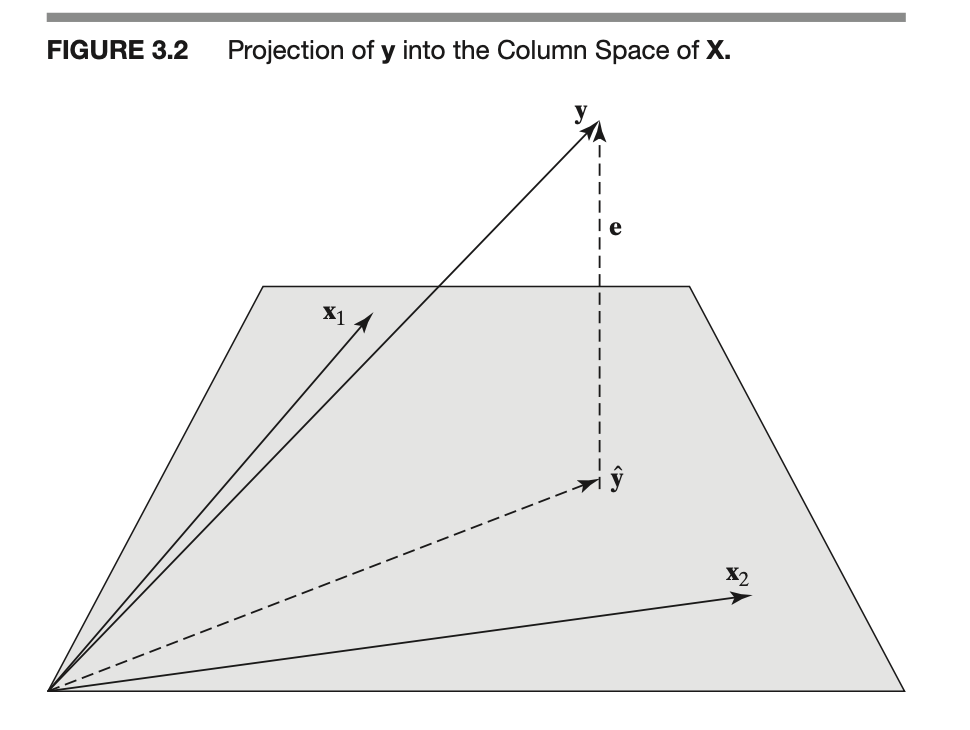
\includegraphics[scale=0.5]{plots/projecao.png}
\end{frame}

\begin{frame}{Fórmula da inversa particionada}
	\begin{itemize}
		\item 		Suponha que particionemos a matriz $\boldsymbol{X} = \begin{bmatrix}
			\boldsymbol{X}_1 & \boldsymbol{X}_2
		\end{bmatrix}$ onde $\boldsymbol{X}_1$ e $\boldsymbol{X}_2$ são matrizes de dimensão $n \times k_1$ e $n \times k_2$.
		\item Nesse caso, a fórmula da inversa particionada nos indica que:
		
	
	\begin{equation*}
			\footnotesize
		\begin{aligned}
			 (\boldsymbol{X}'\boldsymbol{X})^{-1} = \begin{bmatrix}
				\boldsymbol{X_1}'\boldsymbol{X}_1 & 	\boldsymbol{X_1}'\boldsymbol{X}_2 \\
				\boldsymbol{X_2}'\boldsymbol{X}_1 & 	\boldsymbol{X_2}'\boldsymbol{X}_2
			\end{bmatrix}^{-1} =\\  \begin{bmatrix}
				(\boldsymbol{X}_1'\boldsymbol{X}_1)^{-1}  + 	(\boldsymbol{X}_1'\boldsymbol{X}_1)^{-1} \boldsymbol{X}_1'\boldsymbol{X}_2\boldsymbol{F}\boldsymbol{X}_2'\boldsymbol{X}_1 (\boldsymbol{X}_1'\boldsymbol{X}_1)^{-1} & -  (\boldsymbol{X}_1'\boldsymbol{X}_1)^{-1} \boldsymbol{X}_1'\boldsymbol{X}_2\boldsymbol{F}\\
				- \boldsymbol{F}\boldsymbol{X}_2'\boldsymbol{X}_1(\boldsymbol{X}_1'\boldsymbol{X}_1)^{-1} & \boldsymbol{F}\end{bmatrix}
		\end{aligned}
	\end{equation*}
	onde $\boldsymbol{F}=(\boldsymbol{X}_2'\boldsymbol{X}_2 - \boldsymbol{X}_2'\boldsymbol{X}_1(\boldsymbol{X}_1'\boldsymbol{X}_1)^{-1} \boldsymbol{X}_1'\boldsymbol{X}_2 )^{-1} = (\boldsymbol{X}_2'\boldsymbol{M}_1 \boldsymbol{X}_2)^{-1}$ onde $\boldsymbol{M}_1$ é a residualizadora de $\boldsymbol{X}_1$.
\begin{itemize}
	\item Inversa de $\boldsymbol{X}_2'\boldsymbol{M}_1 \boldsymbol{X}_2$  existe pois matriz $\boldsymbol{X}$ tem posto cheio.
\end{itemize}
\end{itemize}

\end{frame}

\begin{frame}{Teorema de Frisch-Waugh-Lovell}
\begin{itemize}
 	\item Da propriedade anterior, segue o importante resultado abaixo:
\end{itemize}
	\begin{theorem}[Frisch-Waugh-Lovell]
		Seja $\hat{b} = \begin{bmatrix}
			\hat{b}_1 \\
			\hat{b}_2
		\end{bmatrix}$. Então:
	$$\hat{b}_2 = \left(\boldsymbol{X}_2'M_1\boldsymbol{X}_2\right)^{-1}\left(\boldsymbol{X}_2'M_1\boldsymbol{y}\right) = \left((M_1\boldsymbol{X}_2)'(M_1\boldsymbol{X}_2)\right)^{-1}\left((M_1\boldsymbol{X}_2)'(M_1\boldsymbol{y})\right) $$ 
	\end{theorem}
\begin{itemize}
	\item Resultado acima nos mostra que estimadores de MQO associados a $\boldsymbol{X}_2$ em uma regressão que inclui $\boldsymbol{X}_1$ e $\boldsymbol{X}_2$ são idênticos a:
	\begin{itemize}
		\item Regredir $\boldsymbol{y}$ em $\boldsymbol{X}_1$, e guardar os resíduos $\boldsymbol{e}_y$.
		\item Para cada $j=1,\ldots k_2$, regredir a $j$-ésima coluna de $\boldsymbol{X}_2$ em $\boldsymbol{X}_1$, e guardar os resíduos ${\boldsymbol{e}_j}$.
		\item Regredir $\boldsymbol{e}_y$ em $\boldsymbol{e}_1,\ldots \boldsymbol{e}_{k_2}$ e recuperar os coeficientes.
	\end{itemize}
\end{itemize}
\end{frame}

	\begin{transitionframe}
	\centering
	\Huge{MQO: Propriedades Estatísticas em Amostras Finitas}
	


\end{transitionframe}
	\begin{frame}{Regressores fixos}
	\begin{itemize}
		\item Nesta seção, analisaremos as propriedades de risco do estimador de MQO.
		\item Essas propriedades serão analisadas com respeito à distribuição de $\boldsymbol{y}$ condicionalmente a $\boldsymbol{X}$.
		\begin{itemize}
			\item Em outras palavras, estamos pensando nas propriedades do estimador sob amostras repetidas (realizações alternativas da incerteza) em que o valor dos regressores é o mesmo da amostra observada.
			\item Ou seja, estamos efetivamente tratando os regressores como fixos sob amostras repetidas.
			\item \textbf{Exemplo:} se $Y_i$ é a taxa de inflação no período $i$, e $X_i$ a taxa de desemprego no período $i-1$, analisaremos as propriedades dos estimadores sob realizações alternativas do cenário econômico em que a taxa de desemprego é igual à observada nos períodos $i=1,\ldots,n$.  
		\end{itemize}
		
	\end{itemize}
\end{frame}

\begin{frame}{Não viés}
\begin{itemize}
	\item Sob a restrição de que:
\begin{assumption}[H2-EXOGENEIDADE]
	$$\mathbb{E}[\boldsymbol{\epsilon}|\boldsymbol{X}]=0$$
	\end{assumption}
	\item O estimador de MQO é não viciado para $\beta$, isto é, qualquer que seja o valor de $\beta \in \mathbb{R}^k$, temos que:
	
	\begin{equation*}
	\mathbb{E}[\hat{b}|\boldsymbol{X} ]= (\boldsymbol{X}'\boldsymbol{X})^{-1}\boldsymbol{X}'\mathbb{E}[\boldsymbol{y}|\boldsymbol{X}] =\beta + (\boldsymbol{X}'\boldsymbol{X})^{-1}\boldsymbol{X}'\mathbb{E}[\boldsymbol{\epsilon}|\boldsymbol{X}]  = \beta 
	\end{equation*}
		\item Observe que a condição de exogeneidade implica que:
	
	$$\mathbb{E}[\boldsymbol{y}|\boldsymbol{X}] = \boldsymbol{X}\beta $$
\end{itemize}
\end{frame}
\begin{frame}{Interpretação da condição de exogeneidade}
\begin{itemize}


		\item Sob amostragem aleatória de uma população, i.e. $(X_i,Y_i)\overset{iid}{\sim}(X,Y)$, condição implica $\mathbb{E}[Y_i|\boldsymbol{X}] = \mathbb{E}[Y_i|X_i] = X_i'\beta \implies \mathbb{E}[Y|X]=X'\beta$.
		\begin{itemize}
			\item A esperança condicional das variáveis $(Y,X)$ que representam a distribuição das características na população de interesse é linear em $X$, {\color{green}e coincide com o modelo linear de interesse}.
				\item Se o modelo postulado é {\color{blue}preditivo}, isso signifca que o parâmetro-alvo do melhor preditor linear consiste também no melhor preditor dentro das funções não lineares de $X$ (ou, de modo equivalente, a melhor aproximação linear a $\mathbb{E}[Y|X]$ é exata).
				\item Se modelo postulado é {\color{blue}causal}, isso significa que as causas não observadas $\epsilon$ apresentam o mesmo valor médio nas diferentes subpopulações definidas pelos valores de $X$. Trata-se de condição mais forte que (i.e. que implica) a condição de identificação $\operatorname{cov}(X,\epsilon) = 0$.
		\end{itemize}
					\item Quando as observações $(X_i,Y_i)$  apresentam dependência entre si, esta condição impõe restrições adicionais.
					\begin{itemize}
						\item Por exemplo, se as observações estão ordenadas no tempo e o modelo postulado é causal, $\mathbb{E}[\epsilon_i|\boldsymbol{X}]=0$ implica que causas não observadas  do fenômeno no período $i$ não exibem associação sistemática com as causas em $i$ {\color{red}e em nenhum outro período}.
						\begin{itemize}
							\item Nesse caso, condição limita retroalimentação entre causas observadas e não observadas no tempo.
						\end{itemize}
					\end{itemize} 
	\end{itemize}

\end{frame}
\begin{frame}{Viés de variável omitida}
\begin{itemize}
	\item Considere um modelo da forma:
	$$\boldsymbol{y}= \boldsymbol{X}_1 \beta_1 + \boldsymbol{X}_2 \beta_2 + \boldsymbol{\epsilon}\, ,$$
	em que $\mathbb{E}[\boldsymbol{\epsilon}|\boldsymbol{X}_1,\boldsymbol{X}_2] = 0$. 
	\begin{itemize}
		\item Por exemplo, num modelo causal, é suficiente observar as causas $\boldsymbol{X}_1$ e $\boldsymbol{X}_2$ para que as causas não observadas restantes estejam balanceadas nas subpopulações definidas pelos valores de $(\boldsymbol{X}_1,\boldsymbol{X}_2)$.
	\end{itemize}
	\item Suponha que você {\color{red}não observe ou desconsidere} $\boldsymbol{X}_2$, e considere o estimador de MQO $\tilde{b}_1$ de $\boldsymbol{y}$ em $\boldsymbol{X}_1$.
	\begin{itemize}
		\item Sob quais condições esse estimador é não viciado para $\beta_1$?
	\end{itemize}
	\item Um cálculo simples nos mostra que:
	\begin{equation*}
		\begin{aligned}
		\tilde{b}_1 = (\boldsymbol{X}_1'\boldsymbol{X}_1)^{-1}\boldsymbol{X}_1'\boldsymbol{y} = \beta_1 + (\boldsymbol{X}_1'\boldsymbol{X}_1)^{-1}\boldsymbol{X}_1' \boldsymbol{X}_2 \beta_2 +(\boldsymbol{X}_1'\boldsymbol{X}_1)^{-1}\boldsymbol{X}_1'\boldsymbol{\epsilon}  \\
		\tilde{b}_1 = \beta_1 + \hat{\gamma}\beta_2 + (\boldsymbol{X}_1'\boldsymbol{X}_1)^{-1}\boldsymbol{X}_1'\boldsymbol{\epsilon} \, ,
		\end{aligned}
	\end{equation*}
	onde $\hat{\gamma}$ é uma matrix $k_1\times k_2$ em que cada coluna representa os coeficientes do estimador de MQO da $j$-ésima coluna de $\boldsymbol{X}_2$ em $\boldsymbol{X}_1$.
	
\end{itemize}
\end{frame}

\begin{frame}{Viés de variável omitida (cont.)}
	\begin{itemize}
		\item Da propriedade da torre, temos que $\mathbb{E}[\boldsymbol{\epsilon}|\boldsymbol{X}_1] = \mathbb{E}[\mathbb{E}[\boldsymbol{\epsilon}|\boldsymbol{X}_1,\boldsymbol{X}_2] |\boldsymbol{X}_1] =0$. Portanto, temos que:
		$\mathbb{E}[\tilde{b}_1|\boldsymbol{X}_1]= \beta_1 + \mathbb{E}[\hat{\gamma}|\boldsymbol{X}_1]\beta_2$

	\item Se uma das duas condições abaixo for satisfeita, estimador será não viciado para $\beta_1$:
			\end{itemize}
	\begin{enumerate}
		\item $\beta_2=0$.
		\begin{itemize}
			\item Se o modelo postulado é causal, essa hipótese significa que as variáveis $\boldsymbol{X}_2$ não possuem efeito causal sobre $\boldsymbol{y}$.
			\item Se o modelo postulado é preditivo,  essa hipótese significa que as variáveis $\boldsymbol{X}_2$ não possuem informação preditiva sobre $\boldsymbol{y}$, uma vez que usamos $\boldsymbol{X}_1$ na predição.
			\begin{itemize}
				\item Nesse caso, estimador de MQO do melhor preditor linear que inclui $\boldsymbol{X}_2$  produzirá, em média, o mesmo resultado que o estimador que inclui $\boldsymbol{X}_1$ e $\boldsymbol{X}_2$.
			\end{itemize}
		\end{itemize}
		\item $\mathbb{E}[\hat{\gamma}|\boldsymbol{X}_1]=0$.
		\begin{itemize}
			\item Essa hipótese é satisfeita se as variáveis em $\boldsymbol{X}_1$ não possuem capacidade preditiva sobre nenhuma das variáveis em $\boldsymbol{X}_2$.
		\end{itemize}
	\end{enumerate}

\end{frame}

\begin{frame}{Estimador linear}
\begin{itemize}
	\item Para obter propriedades de otimalidade para o estimador de MQO, necessitamos introduzir definições adicionais.
	\item Um estimador do parâmetro $\beta$ é dito {\color{red}linear} (em $\boldsymbol{y}$) se:
	
	$$\phi(\boldsymbol{X},\boldsymbol{y}) = A(\boldsymbol{X})\boldsymbol{y}\,,$$
	onde $A: \mathbb{R}^{n\times k} \mapsto \mathbb{R}^{k\times n}$.
	\begin{itemize}
		\item Note que o estimador de MQO é um estimador linear.
	\end{itemize}
	
	
\end{itemize}
\end{frame}

\begin{frame}{Homocedasticidade}
	\begin{itemize}
		\item O estimador de MQO terá propriedades de otimalidade se, além de $H1$-$H2$ restringirmos que:
	\end{itemize}
	\begin{assumption}[H3-Homocedasticidade]
		Existe $\sigma^2 > 0$ tal que $\mathbb{V}[\boldsymbol{\epsilon}|\boldsymbol{X}] = \sigma^2 \mathbb{I}_{n\times n}$.
	\end{assumption}
	\begin{itemize}
		\item A hipótese de homocedasticidade requer que condicionalmente a $\boldsymbol{X}$ os termos de erro $\epsilon_i$, $\epsilon_j$, $j \neq i$, sejam não correlacionados e exibam variância idêntica {\color{red}e não dependente do valor de $\boldsymbol{X}$}.
		\begin{itemize}
			\item Sob  amostragem aleatória de uma população $(X,Y)$ em que vale para o modelo postulado que $\mathbb{E}[\epsilon|X]=0$ (H2), temos que, para $i\neq j$, $\operatorname{cov}(\epsilon_i,\epsilon_j|\boldsymbol{X}) = \mathbb{E}[\epsilon_i\epsilon_j|\boldsymbol{X}]  =\mathbb{E}[\epsilon_i\epsilon_j|X_i, X_j] = \mathbb{E}[\mathbb{E}[\epsilon_i|\epsilon_j, X_i, X_j]\epsilon_j|X_i, X_j] =    \mathbb{E}[\mathbb{E}[\epsilon_i|X_i]\epsilon_j|X_i, X_j] = 0$. Portanto, o requerimento de não covariância condicional não impõe restrições adicionais a H2.
			\item Por outro lado, nesse caso, a hipótese impõe que $\mathbb{V}[Y|X] =\mathbb{V}[\epsilon|X] = \sigma^2$, i.e. que a dispersão de $Y$ nas subpopulações definidas pelos diferentes valores de $X$ sejam as mesmas.
		\end{itemize}
	\end{itemize}
\end{frame}

\begin{frame}{Teorema de Gauss-Markov}
	\begin{itemize}
		\item Defina o seguinte conjunto de distribuições condicionais de $\boldsymbol{y}$ dado $\boldsymbol{X}$:
		$$\small \mathcal{F}(\boldsymbol{X}) = \{P_{\boldsymbol{y}|\boldsymbol{X}}: \exists \delta \in \mathbb{R}^k,  \mathbb{E}_{P_{\boldsymbol{y}|\boldsymbol{X}}} [\boldsymbol{y}|\boldsymbol{X}] = \boldsymbol{X}\delta, \exists \sigma^2 > 0, \mathbb{V}_{P_{\boldsymbol{y}|\boldsymbol{X}}}[ y|\boldsymbol{X}] = \sigma^2 \mathbb{I}_{n\times n}\}$$
		\item Essa é a classe de distribuições condicionais de $\boldsymbol{y}$ dado $\boldsymbol{X}$ em que a esperança condicional é linear em $\boldsymbol{X}$ e a hipótese de homocedasticidade é satisfeita.
		\begin{itemize}
			\item Denote, para uma distribuição condicional $F \in \mathcal{F}(\boldsymbol{X}) $, $\delta(F)$ o parâmetro que entra na esperança condicional.
		\end{itemize}
		\item Com base nas definições acima, temos o seguinte resultado.
		\begin{theorem}[Gauss-Markov]
		 Sob $H1$, o estimador de MQO é o estimador {\color{red}linear} não viciado para $\delta(F)$ de variância uniformemente mínima na classe $\mathcal{F}(\boldsymbol{X})$, i.e. para qualquer outro estimador  {\color{red}linear} $\psi$ tal que $\mathbb{E}_{F}[\psi|\boldsymbol{X}] = \delta(F)$ para todo $F \in \mathcal{F}(\boldsymbol{X})$, temos que, para todo $F \in \mathcal{F}(\boldsymbol{X})$:
			
			$$\mathbb{V}_{F}(\psi|\boldsymbol{X}) - \mathbb{V}_{F}(\hat{b}|\boldsymbol{X})\, \quad \text{é positiva semidefinida} $$
		\end{theorem}
	\end{itemize}
\end{frame}

\begin{frame}{Etapas da demonstração}
	\begin{enumerate}
		\item Mostrar que $\{\delta(F): F \in \mathcal{F}(\boldsymbol{X})\} = \mathbb{R}^k$.
		\begin{itemize}
		\item Basta considerar, para $\delta  \in \mathbb{R}^k$, $ \boldsymbol{y} = \boldsymbol{X}\delta + \boldsymbol{\epsilon}$, com   $\boldsymbol{\epsilon}\sim \mathcal{N}(0, \mathbb{I}_{n\times n})$ e $\boldsymbol{\epsilon}$ independente de $\boldsymbol{X}$.
		\end{itemize}
		\item Com base no resultado acima, mostrar que qualquer estimador linear $A(\boldsymbol{X})\boldsymbol{y}$ não viciado em $\mathcal{F}(\boldsymbol{X})$ deve satisfazer 
		$$A(\boldsymbol{X})\boldsymbol{X} = \mathbb{I}_{k\times k}$$
		
		\item Mostrar que, para todo $F \in \mathcal{F}(\boldsymbol{X})$, $\operatorname{cov}_F(A(\boldsymbol{X})\boldsymbol{y}-\hat{b},\hat{b}|\boldsymbol{X}) = 0_{k\times k}$
		\item Concluir que, para todo $F \in \mathcal{F}(\boldsymbol{X})$: $$\mathbb{V}_F(A(\boldsymbol{X})\boldsymbol{y} -\hat{b}|\boldsymbol{X} ) = \mathbb{V}_F(A(\boldsymbol{X})\boldsymbol{y}|\boldsymbol{X} )-\mathbb{V}_F(\hat{b}|\boldsymbol{X} )$$
	\end{enumerate}
\end{frame}

\begin{transitionframe}
	\centering
	\Huge{MQO: Inferência em Amostra Finita}
	
	
\end{transitionframe}

\begin{frame}{O problema de teste de hipóteses}
	\begin{itemize}
		\item Seja $(\Omega, \Sigma, P)$ um experimento estatístico, e $\mathcal{P}$ um \emph{modelo}.
		\item Sejam $\mathcal{P}_0$ e $\mathcal{P}_1$ uma partição de $\mathcal{P}$.
		\item O problema de decisão estatística conhecido como teste de hipóteses consiste em afirmar se:
				\vspace{-1em}
		$$ P \in \mathcal{P}_0$$
		ou
		$$P \in \mathcal{P}_1$$
		\vspace{-1em}
		\begin{itemize}
			\item Classe $\mathcal{P}_0$ é conhecida como hipótese nula ($H_0$), e $\mathcal{P}_1$ é a classe de alternativas ou hipótese alternativa ($H_1$).
		\end{itemize}
		\item Um {\color{blue}teste } não aleatorizado é uma regra de decisão $\phi:\Omega \mapsto  \{0,1\}$  mensurável (i.e. $\phi^{-1}(\{1\}) \in \Sigma$).
		
		\begin{itemize}
			\item Se $\omega \in \Omega$ observado é tal que $\phi(\omega) = 1$, afirmamos $H_1$ (rejeitamos $H_0$), concluindo por $P\in \mathcal{P}_1$.
			\item Por outro lado, se  $\phi(\omega) = 0$, afirmamos $H_0$ (não rejeitamos $H_0$), concluindo por $P\in \mathcal{P}_0$.
			\begin{itemize}
				\item Em contraste, em testes aleatorizados, permitimos que a hipótese nula seja rejeitada com uma probabilidade dada por $\phi(\omega) \in [0,1]$.
			\end{itemize}
		\end{itemize}
	\end{itemize}
\end{frame}

\begin{frame}{Nível de significância, tamanho e poder }
\begin{itemize}
	\item A princípio, a definição de teste não restringe o comportamento do procedimento estatístico adotado.
	\item Entretanto, gostaríamos de procedimentos estatísticos que limitassem o {\color{blue}erro tipo 1} de se rejeitar a hipótese nula, caso ela seja verdadeira.
	\item Especificamente, para um dado {\color{blue}nível de significância} $\alpha \in [0,1]$, gostaríamos de que o teste satisfizesse:
	$$\mathbb{E}_F[\phi] \leq \alpha,\quad \forall F \in \mathcal{P}_0$$
	\vspace{-1em}
	\begin{itemize}
		\item Probabilidade \textit{ex-ante} de rejeição está limitada a uma probabilidade $\alpha$.
		\item À quantidade $\sup_{F \in \mathcal{P}_0} \mathbb{E}_F[\phi]$ damos o nome de {\color{blue}tamanho} de um teste.
	\end{itemize}
	\item Por outro lado, dado um procedimento que controla o nível de significância, gostaríamos de maximizar {\color{blue}o poder do teste}, i.e., para todo $G \in \mathcal{P}_1$, gostaríamos de tornar:
	$$\nu(G)\coloneqq \mathbb{E}_G[\phi]$$
	o mais alto possível.
	\begin{itemize}
		\item Maximizar o poder é equivalente a minimizar {\color{blue}erro tipo 2} de se afirmar a hipótese alternativa quando ela é falsa.
		\item Usualmente, isso requer que $\sup_{F \in \mathcal{P}_0} \mathbb{E}_F[\phi] = \alpha$.
	\end{itemize}
\end{itemize}
\end{frame}

\begin{frame}{Inferência no modelo linear}
\begin{itemize}
	\item Retomemos o modelo linear visto anteriormente:
$$\boldsymbol{y} =\boldsymbol{X}\beta + \boldsymbol{\epsilon}\, ,$$
onde $\beta$ é desconhecido.
\item Para testes de hipótese em amostras finitas, requeremos:
\begin{assumption}[H5-Normalidade]
$$\boldsymbol{\epsilon}|\boldsymbol{X}\sim \mathcal{N}(0,\sigma^2 \mathbb{I}_{n\times n})$$.
\end{assumption}
\item Hipótese não só requer que erro tenha média condicional zero e matriz de variância homocedástica, mas impõe normalidade da distribuição condicional.
\begin{itemize}
	\item Como parâmetros da normal não dependem de $\boldsymbol{X}$, hipótese implica que $\boldsymbol{\epsilon}$ é independente de $\boldsymbol{X}$.
\end{itemize}
\item Classe de distribuições condicionais compatíveis com a hipótese são:
$$\mathcal{F}^N(\boldsymbol{X}) = \{\boldsymbol{P}_{\boldsymbol{y}|\boldsymbol{X}}: \boldsymbol{y}|\boldsymbol{X}\sim N(\boldsymbol{X}\delta, \sigma^2 \mathbb{I}_{n\times n}),\quad \delta \in \mathbb{R}^k, \sigma^2>0\}$$ 
\end{itemize}
\end{frame}

\begin{frame}{Estatística $F$}
	\begin{itemize}
		\item Suponha que desejássemos testar:
		\vspace{-0.5em}
		$$H_0: R\beta = c$$
		\vspace{-0.5em}
		contra a  alternativa
\vspace{-0.5em}
		$$H_1: R\beta \neq c$$
		onde $R$ é uma matriz $q \times k$ de posto $q$, e $c$ é uma vetor $q \times 1$.
		\begin{itemize}
			\item $H_0$ e $H_1$ formam partição de $\mathcal{F}^{N}(\boldsymbol{X})$
		\end{itemize}
		\item Considere a seguinte estatística de teste:
\end{itemize}
\vspace{0.8em}
		$$\footnotesize W_{R,c} = \frac{(R\hat{b}-c)'\left(R\hat{\sigma}^2(\boldsymbol{X}'\boldsymbol{X})^{-1}R'\right)^{-1}(R\hat{b}-c)}{k}  = \frac{(R\hat{b}-c)'\left(R(\boldsymbol{X}'\boldsymbol{X})^{-1}R'\right)^{-1}(R\hat{b}-c)}{k \hat{\sigma}^2}\, ,$$
	
		\begin{itemize}
			\item $\hat{\sigma}^2 = \frac{1}{n-k}\sum_{i=1}^n (Y_i -X_i'\hat{b})^2$, com $\hat{\sigma}^2 (\boldsymbol{X}'\boldsymbol{X})^{-1}$ é estimador de $\mathbb{V}[\hat{b}|\boldsymbol{X}]$.
			\item Estatística mede o desvio de $R\hat{b}$ a $c$, onde a distância é ``ponderada'' pelo inverso da variância de  $R\hat{b}$.
			\item Valores grandes da estatística formam evidência contra hipótese nula.
		\end{itemize}

\end{frame}

\begin{frame}{Distribuição da estatística de teste, sob a hipótese nula}
\begin{proposition}
	Suponha válidas as Hipóteses 1 e  4. Se a distribuição $\mathbb{P}$ satisfaz a hipótese nula, então:
	
	$$W_{R,c}|\boldsymbol{X}\sim F(k,n-k)$$
\end{proposition}
\begin{itemize}
	\item Etapas para demonstração do resultado:
	\begin{enumerate}
		\item Mostrar que, sob a nula, $N := (R\hat{b}-c)'\left(R\sigma^2(\boldsymbol{X}'\boldsymbol{X})^{-1}R'\right)(R\hat{b}-c) \sim \chi^2(k)$.
		\item Mostrar que $(n-k)\hat{\sigma}^2/\sigma^2 \sim \chi^2(n-k)$.
		\item Mostrar que $N$ e $\hat{\sigma}^2$ são independentes.
	\end{enumerate}
\end{itemize}
\end{frame}

\begin{frame}{Teste de hipótese}
\begin{itemize}
	\item O resultado anterior sugere considerar a seguinte regra de decisão, para um nível de significância $\alpha \in [0,1]$:
	$$\phi \coloneqq \mathbf{1}\{W_{R,c}> q_F(1-\alpha|k,n-k)\}$$
	onde $q_F(1-\alpha|k,n-k)$ é o quantil $1-\alpha$ da distribuição $F(k,n-k)$.
	\begin{itemize}
		\item Rejeitamos a nula se $W_{R,q}$ for suficientemente alta.
		\item Com base no \textit{slide} anterior, se nula for verdadeira, tem-se $\mathbb{E}[\phi|\boldsymbol{X}] = \alpha$.
	\end{itemize}
	\item Estatística $W_{r,c}$ pode ser reescrita a partir da diferença relativa entre o $R^2$ do estimador de MQO irrestrito, relativamente ao estimador de MQO que impõe a hipótese nula.
	\begin{itemize}
		\item Veja o livro do Greene para detalhes.
	\end{itemize}
	\item No caso em que $q=1$, teste é equivalente a rejeitar a nula se:
	$$|\hat{t}_{R,q}| > q_t(1-\alpha/2|n-k)$$
	onde $q_t(1-\alpha/2|n-k)$ é o quantil $1-\alpha/2$ de uma t de Student com $n-k$ graus de liberdade, e:
	\vspace{-0.5em}
	$$\hat{t}_{R,c} = \frac{(R\hat{\beta}-c)}{R\hat{\sigma}^2(\boldsymbol{X}'\boldsymbol{X})^{-1}R'}$$
\end{itemize}
\end{frame}



\end{document}



\begin{transitionframe}
	\centering
	\Huge{MQO: Propriedades Assintóticas}
	
	
\end{transitionframe}
